% !Mode:: "TeX:UTF-8"
\documentclass[notheorems,serif]{beamer}

%选用主题
\usetheme{Rochester}
%\usetheme{default}
%\usetheme{AnnArbor}
%\usetheme{Antibes}
%\usetheme{Bergen}
%\usetheme{Berkeley}
%\usetheme{Berlin}
%\usetheme{Boadilla}
%\usetheme{CambridgeUS}
%\usetheme{Copenhagen}
%\usetheme{Darmstadt}
%\usetheme{Dresden}
%\usetheme{Frankfurt}
%\usetheme{Goettingen}
%\usetheme{Hannover}
%\usetheme{Ilmenau}
%\usetheme{JuanLesPins}
%\usetheme{Luebeck}
%\usetheme{Madrid}
%\usetheme{Malmoe}
%\usetheme{Marburg}
%\usetheme{Montpellier}
%\usetheme{PaloAlto}
%\usetheme{Pittsburgh}
%\usetheme{Rochester}
%\usetheme{Singapore}
%\usetheme{Szeged}
%\usetheme{Warsaw}

% As well as themes, the Beamer class has a number of color themes
% for any slide theme. Uncomment each of these in turn to see how it
% changes the colors of your current slide theme.

%\usecolortheme{albatross}
\usecolortheme{beaver}
%\usecolortheme{beetle}
%\usecolortheme{crane}
%\usecolortheme{dolphin}
%\usecolortheme{dove}
%\usecolortheme{fly}
%\usecolortheme{lily}
%\usecolortheme{orchid}
%\usecolortheme{rose}
%\usecolortheme{seagull}
%\usecolortheme{seahorse}
%\usecolortheme{whale}
%\usecolortheme{wolverine}

%设置被cover的内容不显示
%\setbeamercovered{transparent}

\useinnertheme{rounded}
\usecolortheme{default}



%调用包
\usepackage[no-math, cm-default]{fontspec}
\usepackage{xltxtra}
\usepackage{xunicode}   
\usepackage{xcolor}
\usepackage{amsmath,amssymb}
\usepackage{multimedia}
\usepackage{subfigure}
\usepackage{animate}
\usepackage{multirow}
\usepackage{slashbox}
\usepackage{algorithm}
\usepackage{algorithmic}
\usepackage{xkeyval}
\usepackage{todonotes}
\presetkeys{todonotes}{inline}{} 
\usepackage{multicol}
\usepackage{changes}
\usepackage{fancybox}
%\usepackage{lipsum}% <- For dummy text
\definechangesauthor[name={Huayi Wei}, color=red]{why}

\renewcommand{\algorithmicrequire}{\textbf{INPUT:}}
\renewcommand{\algorithmicensure}{\textbf{OUTOUT:}}
\makeatletter
\renewcommand*\env@matrix[1][\arraystretch]{%
  \edef\arraystretch{#1}%
  \hskip -\arraycolsep
  \let\@ifnextchar\new@ifnextchar
  \array{*\c@MaxMatrixCols c}}
\makeatother


\input{pptheader.tex}


\begin{document}

\title[]{The surface finite element method for pattern formation on evolving biological surfaces}
\author[M. Liu]{Jianggang Liu\\
\medskip
Advisor: Huayi Wei and Kai Jiang}
\institute[XTU]{
\vspace{5pt}
School of Mathematics and Computational Science\\
 Xiangtan University
\vspace{0.5cm}
}
\date{\today}

%\pgfdeclareimage[height=1cm]{institution-logo}{figures/xtu.pdf}
%
%\logo{\pgfuseimage{figures/xtu.pdf}}

\frame[plain]{\titlepage}


\AtBeginSection[]{

  \frame<beamer>{ 

    \frametitle{Outline}   

    \tableofcontents[currentsection] 

  }
}



% Introduce backgroud knowledge
\section{Backgroud}


\section{Numerical Results}

\begin{frame}
\frametitle{Efficiency of the Numerical Method}

\begin{table}[H]
\caption{
$\chi N=30,f=0.2$, $\Gamma=2.9$.}
  \label{tab:refinemesh}
  \centering
\small
\begin{tabular}{|c|c|c|c|c|c|}
 \hline
 \# of Node  & \# of Elem. & $\Gamma$ & $\Gamma$-diff. & Hamiltonian &
 Ham. diff. \\
 \hline
162  & 320   & -  & - & -&  -  \\ 
 \hline
 642   & 1280  & 3.7071  & 8.071e-1 & -3.172693  & - \\
 \hline
2562  & 5120  & 3.5786  & 1.285e-1 & -3.160542 &  1.215e-2\\
 \hline
10242 & 20480 & 3.5656  & 1.129e-2 & -3.165431 & 4.889e-3\\
 \hline
40962 & 81920 & 3.5632  & 2.399e-3 & -3.166846 & 1.415e-3 \\
 \hline
\end{tabular}
\end{table}

\begin{figure}
    \centering
    \subfigure[]{\includegraphics[scale=0.27]{figures/mesh/s3-1.pdf}}
    \hspace{0.5cm}
    \subfigure[]{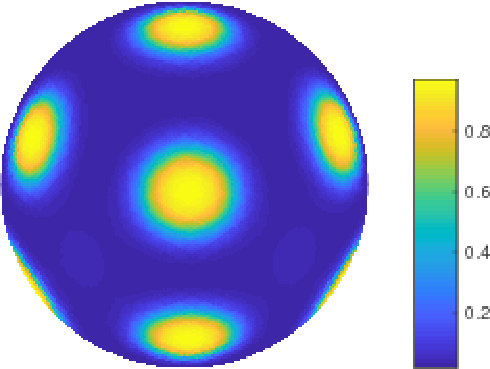
\includegraphics[scale=0.27]{figures/mesh/s4-3.pdf}}
    \hspace{0.5cm}
    \subfigure[]{\includegraphics[scale=0.27]{figures/mesh/s51-crop.pdf}}
    \hspace{0.5cm}
    \subfigure[]{\includegraphics[scale=0.27]{figures/mesh/s61-crop.pdf}}
\end{figure}


\end{frame}


\begin{frame}
\frametitle{ Previous and Our Work}
    \begin{itemize}

\item Many numerical methods of the SCFT model have been developed on flat
    spaces, however, only few work focus on designing the numerical methods on
            curved surfaces ([Chantawansri et al. 2007], [Li, Liang et al. 2014], [Li et al. 2006, 2014], etc).

\medskip
    
\item We develop a computational method of self-assembled phases of block
    copolymers on a general curved surface based on the self-consistent
            field theory (SCFT), which is discretized by the surface finite element
            method.
\end{itemize}
\end{frame}



\begin{frame}
    \centering{\Large {Thank you!}}
\end{frame}

\end{document}
